%----------------------------------------------------------------------------------------
%    PACKAGES AND THEMES
%----------------------------------------------------------------------------------------

\documentclass[aspectratio=169,xcolor=dvipsnames]{beamer}
\usetheme{SimpleDarkBlue}

\usepackage{hyperref}
\usepackage{graphicx} % Allows including images
\usepackage{booktabs} % Allows the use of \toprule, \midrule and \bottomrule in tables
\usepackage{biblatex}
\addbibresource{mlops.bib}
\graphicspath{{./images/}}
%----------------------------------------------------------------------------------------
%    TITLE PAGE
%----------------------------------------------------------------------------------------

\title{Brute-forcing Monte Carlo Simulation}

\author{Radu Briciu}

\institute
{
	BSc Finance (Hons) \\ 
	University of Westminster \\
	\vspace*{1em}
	City, University of London \\
	Faculty of Finance
}
\date{\today} % Date, can be changed to a custom date

%----------------------------------------------------------------------------------------
%    PRESENTATION SLIDES
%----------------------------------------------------------------------------------------

\begin{document}
	
	\begin{frame}
		% Print the title page as the first slide
		\titlepage
	\end{frame}
	
	\begin{frame}{Overview}
		In this session we explore a proposed method for estimating nonlinear stochastic functions in the context of path dependent financial derivatives
		\tableofcontents
	\end{frame}
	
	%------------------------------------------------
	\section{Some a priori content}
	%------------------------------------------------
	
	\begin{frame}{Financial Derivatives}
		What are financial derivatives?
		\begin{figure}[h]
			\centering
			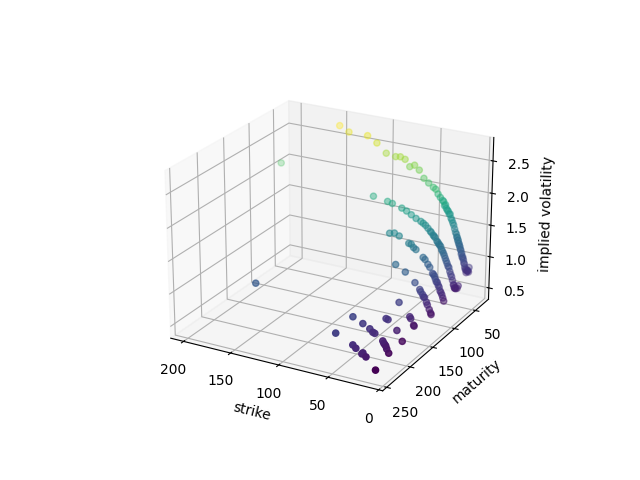
\includegraphics[width=0.5\textwidth]{vix.png}
		\end{figure}
	\end{frame}
	
	\begin{frame}{The Heston Model}
		\begin{align}
			dS_t &= \left( r - \frac{v_t}{2} \right) dt + \sqrt{v_t} \left( \rho dW_t + \sqrt{1 - \rho^2} dB_t \right) \label{eq:hdXt} \\
			dv_t &= \kappa (\theta - v_t) dt + \eta \sqrt{v_t} dW_t \hspace{1.8cm} \label{eq:hdvt}
		\end{align}
	\end{frame}
	
	\begin{frame}{Asian Options}
		\begin{align}
			C^{\text{Arithmetic}}_t &= e^{-r(T-t)} \times \frac{1}{m} \sum_{i=1}^{m} (S_{T}^{\text{Arithmetic}} - K)^{+} \\
			C^{\text{Geometric}}_t &= e^{-r(T-t)} \times \frac{1}{m} \sum_{i=1}^{m} (S_{T}^{\text{Geometric}} - K)^{+}
		\end{align} \label{eq:AsianPayoffs}
	\end{frame}
	
	\begin{frame}{References}
		\nocite{*}
		\printbibliography
	\end{frame}
	
	%------------------------------------------------
	
	\begin{frame}
		\Huge{\centerline{\textbf{The End}}}
	\end{frame}
	
	%----------------------------------------------------------------------------------------
	
\end{document}